\documentclass[12pt, a4paper]{report}
\usepackage[utf8]{inputenc}
\usepackage[left=40mm, right=20mm, top=30mm, bottom=30mm]{geometry}
\usepackage{titlesec}
\usepackage{xparse}
\usepackage{microtype}
\usepackage{graphicx}
\usepackage{amsmath}
\usepackage{amsfonts}
\usepackage{placeins}
\usepackage{tikz}
\usepackage{algorithm}
\usepackage{algpseudocode}
\usepackage{setspace}
\usepackage{parskip}
\usepackage{biblatex} %Imports biblatex package
\addbibresource{bibliography.bib} %Import the bibliography file
\usetikzlibrary{shapes.geometric}

\titleformat{\chapter}[hang]{\Huge\bfseries}{\thechapter}{20pt}{\Huge\bfseries}

\graphicspath{{figures/}}

\NewDocumentCommand{\codeword}{v}{%
\texttt{{#1}}%
}

\renewcommand{\contentsname}{Table of Contents}

\setlength{\parindent}{10pt}
\title{
Designing and Implementing a Tensor Calculus \vspace{50pt}

\normalsize B A C H E L O R ' S $\;$ T H E S I S \vspace{10pt}

In Fulfillment of the Requirements for the Academic Degree of \vspace{10pt}

Bachelor of Science (B.Sc.) \vspace{10pt}

In the Study Program 'Computer Science' \vspace{30pt}

FRIEDRICH SCHILLER UNIVERSITY JENA \vspace{10pt}

Faculty of Mathematics and Computer Science \vspace{60pt}

submitted by Farin Lippmann \vspace{10pt}

born on the 02.02.2000 in Gera \vspace{10pt}

Supervisor: Prof. Dr. Joachim Giesen \vspace{10pt}

}
\date{\normalsize Jena, 25.08.2022}

% Area: Generic optimization
% Topic: Derivatives of higher-order tensor expressions
% Research Question: Can we design and implement an Einstein-notation-based tensor calculus for automatic symbolic differentiation of tensor expressions?

% Related Research: 
% - Matrix Calculus paper (uses ricci notation)
% - Tensor Calculus paper (basis for this thesis)
% - Algebra systems build scalar-valued functions for each tensor entry, inefficient [from Matrix Calculus Paper]

% Questions:
% - What am I improving over Matrix Calculus? 
%   -> Einstein notation instead of Ricci
%   -> Actually works on arbitrary tensor inputs
%   -> Cleanup inbetween derivation steps?
% - Why Einstein over Ricci?
%   -> Ricci is more complex, allows differentiating between tensors and their dual (multilinear maps)
%      which we don't need, tensors are strictly datastructures for us
%   -> Because we don't need the complexities of Ricci, Einstein allows a more elegant internal representation


\begin{document}
\maketitle

\addcontentsline{toc}{chapter}{Abstract}
\chapter*{Abstract}
In optimization problems, derivatives play a crucial role in finding an optimal solution.
Automatic symbolic differentiation of matrix expressions and numerical differentiation of tensor expressions are well researched and used intensively in the industry.
The field of automatic symbolic differentiation of tensor expressions however is not as well explored.
In this thesis, we design and implement a tensor calculus for automatic symbolic differentiation of tensor expressions of any order.
It uses an Einstein-like product notation that is more general than the notation used in the popular Ricci calculus.
\pagenumbering{gobble}

\addcontentsline{toc}{chapter}{Table of Contents}
\tableofcontents
\pagenumbering{arabic}
\setcounter{page}{3}

\chapter{Introduction}

With the rise of machine learning applications, interest in optimization problems has been growing.
In these kinds of problems, one seeks to find values for a number of parameters that maximize or minimize a given objective function.
While some optimization problems have a closed-form solution which can be computed directly, many can only be solved approximately.
When computing these approximate solutions, derivatives play a crucial role.
In particular, the first derivative of the objective function is used in the ubiquitous gradient descent procedure.
In most optimization problems, multiple parameters need to be optimized simultaneously.
This means that derivatives need to be computed with respect to multiple variables, organized either in vectors, matrices or higher-order tensors.
Commonly used machine learning frameworks (like Tensorflow, PyTorch or Theano) focus heavily on the first derivatives of the objective function.

Higher-order derivatives can, however, also be of interest.
As an example, the matrix of second-order partial derivatives, called the Hessian, is used in the application of Newton's method, which can be more efficient than gradient descent for some problems.
Convexity checks constitute another application of higher-order derivatives.
The convexity of objective functions and their associated optimization problems play a major role in the field of optimization.
If a problem is strictly convex or concave, then it has a unique global optimum and the gradient descent algorithm can approximate it arbitrarily well.
To check for convexity, the objective function's Hessian matrix needs to be computed and checked for semidefiniteness.
If the function's inputs are naturally organized in a matrix or higher-order tensor, then the resulting Hessian will also be a higher-order tensor.
The prevalent machine learning frameworks have no way to directly compute these derivatives, and classical computer algebra systems struggle with efficiency, as they work on the level of individual tensor entries.

To bridge this gap, we design and implement a tensor calculus that allows for automatic symbolic differentiation of tensor expressions of any order.
Additionally, this calculus will use an Einstein-like notation to represent tensor products, rather than the more complex notation used in Ricci calculus.

This thesis builds on the work by Laue, Mitterreiter and Giesen, who have built a similar calculus for matrix derivatives \cite{matrixpaper} and developed the theoretical foundation for an Einstein notation based tensor calculus \cite{tensorpaper}.

The structure of the thesis is as follows.
First, we develop the syntax of the calculus in form of a grammar.
Then, we discuss the parsing and representation of tensor expressions.
Following that, we describe the theoretical background and practical implementation of the differentiation process.

\chapter{A Syntax for Tensor Expressions}
\section{Aims}
In this chapter we develop the language that will be used to specify tensor expressions for differentiation.
To differentiate a tensor expression, three pieces of information are needed: 1. the tensor expression itself, 2. the variable with respect to which should be differentiated, 3. the tensor order of all variables in the expression.
The neccessity of the first two is obvious, while the third might not immediately be.
Later, during differentiation, the tensor orders of each subexpression need to be known.
How these are computed from the given tensor orders of variables is covered in chapter 3.

Our aims when developing the syntax are the following.
The syntax should allow representation of tensor expressions of arbitrary order and should be as general as possible.
Even so, as the motivation for this thesis comes from the background of optimization and machine learning, the most common specifics of these fields should be covered.

The main point of interest for this syntax is how to represent tensors and their products, as there are many ways to multiply two tensors.
We start with an established tensor calculus and its notation, and generalize it to fit our problem domain.

\section{Representing Tensor Products}
There exists a calculus for tensor expressions, called Ricci calculus, that is heavily used in physics. %TODO: RICCI REF
The notation it uses allows for tensors to represent both $n$-dimensional arrays and multilinear functions.
The distinction between the two forms occurs by the location of their indices, either in sub- or superscript.
For example, the inner product of two vectors, $y^Tx$, would be written as $y_ix^i$. And the Matrix-vector product $Ax$ would be $A^i_jx^j$.
While Ricci calculus can be useful, for example to physicists, the many indices on each tensor make it less readable.

Since, for our purposes, tensors are simply containers for variables, we have no need to expressly define some tensors as multilinear functions.
A part of Ricci calculus that we bring over into our notation is a derived version of the Einstein summation convention. %TODO: EINSTEIN REF
This is a notational convention that allows elegant representation of tensor products.
Since tensors, depending on their order, may be multiplied in many ways, we need a way to describe which tensor axes should be multiplied in what way.
For example, two vectors could be multiplied by taking their inner product, their outer product, or even their elementwise product.
Einstein notation handles this problem by adding index strings to the inputs and the output of the product, each index representing an axis in the respective tensor.
If an index appears in both inputs, the respective axes will be multiplied.
If an index appears in inputs but not in the output, this axis will be summed over.
In true Einstein-notation, output indices are omitted, so indices that appear in both inputs are always summed over. 
For more generality, we include output indices.
This simple set of rules provides an elegant way to express the main tensor operations.

We take a large part of the syntax for tensor multiplication from the established Python software package \textit{Numpy}, specifically its \codeword{einsum} procedure. %TODO: NUMPY REF
A product of two tensors $x$ and $y$ has the form $x*_{(a,b \rightarrow c)}y$, where $a$,$b$ and $c$ are strings of indices.
A formal characterization of the product $C = A *_{(s_1,s_2 \rightarrow s_3)} B$ is given in Equation \ref{eq:product}, where $s_1$, $s_2$ and $s_3$ represent index sets.
Note that for two index sets $s_1$ and $s_2$, we write $s_1 s_2$ as shorthand for $s_1 \cup s_2$.

\begin{equation}
    C[s_3] = \sum_{(s_1 s_2)  \backslash s_3} A[s_1] \cdot B[s_2]
    \label{eq:product}
\end{equation}

As an example of tensor products, see the inner, outer and elementwise product of two first order tensors (vectors) $x$ and $y$: $x*_{(i,i \rightarrow)}y$, $x*_{(i,j \rightarrow ij)}y$, $x*_{(i,i \rightarrow i)}y$.
The application of a matrix $A$ to a vector $v$ would be written as $A*_{(ij,j \rightarrow i)}v$, while the elementwise product of two matrices $A$ and $B$ would be $A*_{(ij,ij \rightarrow ij)}B$.
By swapping the order of output indices, the axis order can be manipulated.
A special case of this is the matrix transpose, which for a matrix $X$ can be taken using the product $X *_{(ij, \rightarrow ji)} 1$.
One may even take diagonals of tensors using this notation, the inner product of a square matrix $A$'s main diagonal and a vector $v$ would be $A*_{(ii,i \rightarrow)}v$.


\section{Grammar}
With the representation of tensor products handled, we can now define the full syntax grammar.
The grammar, presented here in extended backus-naur form, is based on a standard grammar for mathematical expressions by Julien Klaus. %Todo: Source here?
It was adapted to tensor expressions by generalizing multiplication to tensor products using the einstein summation convention.
\begin{verbatim}
expr = term {( '+' | '-' ) term}+
term = factor {( '*(' productindices ')') factor | '/' factor}+
productindices = tensorindices ',' tensorindices '->' tensorindices
tensorindices = {smallalpha}+
factor = {'-'} atom {'^' ('(' expr ')' | atom)}+
atom = number | function '(' expr ')' | tensorname | '(' expr ')' | 
       delta
number = ['-'] digit* '.' digit* [( 'e' | 'E' ) ['+' | '-'] (digit)*]
digit = [0-9]
function = 'sin' | 'cos' | 'tan' | 'arcsin' | 'arccos' | 'arctan' | 
           'tanh' | 'exp' | 'log' | 'sign' | 'relu' | 'abs' | 'det' | 
           'inv' | 'adj'    
delta = 'delta(' {digit}+ ')' 
\end{verbatim}
Here \texttt{\string{x\string}} describes that \texttt{x} may occur any number of times, while \texttt{\string{x\string}+} lets \texttt{x} appear at least once.

As can be seen in the grammar, we allow the following binary operations on tensors: products (\codeword{*(,->)}), sums (\codeword{+}), differences (\codeword{-}) and quotients (\codeword{/}).
With the exception of tensor products, which have already been discussed, these operations are executed elementwise.
Exponentiation (\codeword{^}) is also included, but not as a true binary operator on tensors, as the exponent may only be scalar, with each entry of the basis tensor being combined with the exponent.
This is not apparent from the grammar, as tensor variable order is specified separately from the tensor expression itself.

A variety of functions with relevance to optimization and machine learning are included, mostly being applied elementwise to tensors of any order.
The exceptions to this are the matrix inverse \codeword{inv}, the matrix determinant \codeword{det} and the adjugate matrix $\codeword{adj}$, all of which are not applied elementwise and may only operate on order 2 tensors.
The inclusion of these functions takes away from the generality of our grammar, as the idea of an inverse and a determinant can only be applied to matrices, not higher-order tensors, but they are crucial to some common optimization problems that work with matrices.

\chapter{Parsing and Representation}
Having defined the syntax, we now discuss how a given tensor expression is parsed and represented internally.
In our application, tensor expressions are represented using directed acyclic graphs derived from binary trees.
This data structure was chosen because graphical representations are well tested for expressions and because the foundational work by Laue, Mitterreiter and Giesen also assumes such a representation.
This allows the differentiation rules stated in their work to be easily implemented.
Furthermore, many of the algorithms described in this chapter and the next are most naturally written recursively.
A recursive data structure like a tree lends itself to these algorithms.
In this chapter we first describe how a tensor expression is parsed into a binary expression tree and explain the processing steps taken to transform the binary tree into a directed acyclic graph without duplicate subexpressions.
We also describe how we assign a tensor order and an axis tuple to each node in the graph, which are required for differentiation and for possible numerical evaluation of the derivative expression.

\section{Parsing}
The process of turning a string into a different data structure that allows for further processing is called parsing.
It is split into two steps, tokenization and tree building.

\subsection{Tokenization}
To be able to parse an expression string, we first transform it into a sequence of tokens.
This is done by the tokenizer, sometimes also called lexical scanner, which recognizes certain defined patterns in the expression string and unifies them into a token.
Each of these tokens represents a logical unit that is used in the next step of parsing.
Tokenization allows the parser to work only with well-defined tokens, not having to work on the level of individual characters.
Each token is made up of two parts, the descriptor and the identifier.
The descriptor is one of a few defined categories, describing what kind of logical unit the token forms, while the identifier contains the characters the token was formed from.
As an example, the string \codeword{A + sin(b)} would be tokenized into the following sequence: \codeword{(ALPHANUM, 'a'), (PLUS, '+'), (ELEMENTWISE_FUNCTION, 'sin'), (LRBRACKET, '('), (LOWERCASE_ALPHA, 'b'), (RRBRACKET, ')')}.

We define token descriptors for constants (\textit{e.g.} \codeword{'1.05'}), variable names (\textit{e.g.} \codeword{'A'}, \codeword{'b'}, \codeword{'C1'}), special symbols (\codeword{'+'}, \codeword{'-'}, \codeword{'*'}, \codeword{'/'}, \codeword{'^'}, \codeword{','}, \codeword{'('}, \codeword{')'}, \codeword{'>'}), keywords (\codeword{'declare'}, \codeword{'expression'}, \codeword{'derivative'}, \codeword{'wrt'}) and function names, which are recognized using the list of functions given in the grammar (\textit{e.g.}  \codeword{'sin'}, \codeword{'abs'}, \codeword{'det'}).
There are two token descriptors for functions, \codeword{ELEMENTWISE_FUNCTION} and \codeword{SPECIAL_FUNCTION}, because derivative rules are different for these two types.
Special functions are the matrix determinant \codeword{det}, the matrix inverse \codeword{inv} and the adjugate matrix \codeword{adj}.

\subsection{Tree Building}
The output of the tokenizer is used to build a binary tree representing the expression.

A binary tree is a type of tree where each node has at most two child nodes.
Like in other trees, each node has exactly one parent node.
The exception to this is the root, which has no parent.
We call nodes that have no children leaf nodes.

Formally, we define a binary tree $B$ as follows:
$B$ is either the empty set or a tuple $(\text{left}(B),\text{root}(B),\text{right}(B))$, where $\text{left}(B)$ and $\text{right}(B)$ are also binary trees and have $B$ as their only parent, and $\text{root}(B)$ is the root of the tree, containing some value.

The process  of constructing such a tree from a given expression follows the structure of the grammar defined in the previous chapter.
Starting with \codeword{expr}, we recursively step through the grammar, using the tokens to decide which options to follow.
For each of the words defined in the grammar there is a function in our parser.
When a certain word is expected, the function is called.
For example, at the start, \codeword{expr} is called, which first calls \codeword{term}, which calls \codeword{factor}, which then looks for any \codeword{MINUS}-tokens before calling \codeword{atom}, which then checks if there is a constant, a function application, a variable name, or another expression, and so forth.
Thus, we traverse the expression from left to right while building binary tree nodes when appropriate.
Leaf nodes are created when we reach constants or variable names, and they are connected using branch nodes containing operators or functions.
Each node, with its subtree, represents a subexpression, with the root node of the whole tree representing the entire expression.
If there is ever a point at which expectations are not met, for example, if a left round bracket token (\codeword{(LRBRACKET, '(')}) is expected but not found, we abort program execution.

As an example, we take the expression from before, \codeword{A + sin(b)}, tokenized to \codeword{(ALPHANUM, 'A'), (PLUS, '+'), (ELEMENTWISE_FUNCTION, 'sin'), (LRBRACKET, '('), (LOWERCASE_ALPHA, 'b'), (RRBRACKET, ')')}.

The order of function calls generated when parsing this expression would be the following:

\begin{itemize}
    \setlength\itemsep{0.01em}
    \item \codeword{expr}
    \item \codeword{term}
    \item \codeword{factor}
    \item \codeword{atom} | We identify \codeword{'A'} as a variable name, generate a leaf node and jump back up the call stack to \codeword{expr}. There, we find the expected \codeword{'+'} and add a sum node as the parent of our leaf node.
    \item \codeword{term}
    \item \codeword{factor}
    \item \codeword{atom} | We identify \codeword{'sin'} as a function name and generate an elementwise-function node as the second child of our sum node. We also find the expected \codeword{'('}.
    \item \codeword{expr}
    \item \codeword{term}
    \item \codeword{factor}
    \item \codeword{atom} | We identify \codeword{'b'} as a variable name and generate another leaf node as the child of our elementwise-function node. We jump back up the call stack, find the expected \codeword{')'}, jump all the way to the top of the call stack and finish.
\end{itemize}

The binary tree generated from this can be seen in Figure \ref{fig:tree_example}.
Note that, by convention, we set the argument of a unary function node to its right child.

\begin{figure}
    \centering
    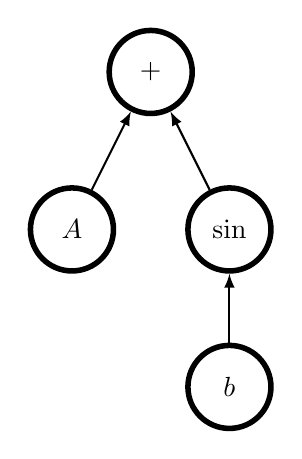
\begin{tikzpicture}[main/.style={draw, circle, minimum size=30pt, line width=2pt}, info/.style={rectangle, rounded corners=5, draw}, n/.style={-latex, line width=0.75pt}, d/.style={-latex, line width=0.75pt, dashed}]
        % nodes
        \node[main] (A) at (0,2) {$A$};
        \node[main] (b) at (2,0) {$b$};
        \node[main] (+) at (1,4) {$+$};
        \node[main] (sin) at (2,2) {$\text{sin}$};
        % edges
        \draw [->, n] (A) -- (+);
        \draw [->, n] (b) -- (sin);
        \draw [->, n] (sin) -- (+);
    \end{tikzpicture}
    \caption{Binary expression tree generated from the expression string \texttt{A + sin(b)}. Empty nodes are omitted.}
    \label{fig:tree_example}
\end{figure}

\section{Preprocessing}
Having shown how a binary expression tree is created from a given tensor expression, we now describe how this tree is processed further to prepare it for differentiation.
We employ the following three preprocessing steps.
\begin{itemize}
    \item Some subtrees are substituted with equivalent ones which are more easily differentiated.
    \item Subtrees which occur more than once are fused.
    \item Each node's output tensor order is determined and stored.
\end{itemize}

\subsection{Equivalent Subtree Substitution}
Some operations or functions may be viewed as equivalent to, or as a special case of another, more easily differentiable operation or function.
In these cases, we substitute the more general case to reduce the number of differentiation rules that need to be implemented.
For example, when encountering the expression $A - B$, we substitute $A + -(B)$, viewing $(-)$ as an elementwise function.
This allows us to use the differentiation rules for sums and elementwise functions, not having to implement a new rule for differences.
A full overview of the substituted expressions can be seen in Table \ref{tab:substitutions}.
\begin{table}[ht]
    \centering
    \begin{tabular}{l | l}
        Original & Substitute \\\hline
        $A-B$ & $A + -(B)$ \\
        $A^B$ & $\text{exp}(B *_{(,->)} \text{log}(A))$ \\ %TODO: Macht 0^B hier Probleme?
        $A/B$ & $A \;.^*\; \text{elementwise\_inverse}(B)$ \\
        $\text{adj(X)}$ & $\text{det}(X) *_{(,ij \rightarrow ij)} \text{inv}(X)$ \\ 
    \end{tabular}
    \caption{Table showing all operations that get substituted during preprocessing, along with their substitutes. Note that $(.^*)$ is a placeholder for elementwise multiplication. It is replaced with the appropriate tensor product during tensor order determination. $\text{elementwise\_inverse}$ is an elementwise function for which a differentiation rule is implemented.}
    \label{tab:substitutions}
\end{table}
\FloatBarrier

\subsection{Common Subtree Elimination}
When differentiating, we need to be able to tell when a subexpression is reached multiple times.
To help with this, and also to reduce the number of nodes in the expression tree, we fuse subtrees that occur more than once.

First, to identify duplicate subtrees, the notion of equality needs to be defined for trees.
We define equality of two trees, $A$ and $B$, as follows.
$$
A = B \iff \text{root}(A) = \text{root}(B) \land \text{left}(A) = \text{left}(B) \land \text{right}(A) = \text{right}(B)
$$
Equality of nodes is handled by comparing all components of the node (node type, name, indices for product nodes) individually.

Now that we may identify when two subtrees are equal, we continue with common subtree elimination.
We first obtain all subtrees by traversing the whole tree.
Then, we store each unique subtree we find in a hash table.
When we encounter a subtree that is already present in our hashmap, we let its parent node have the tree in the hashmap as its child instead of the original.
In doing so, we remove duplicate subtrees and transform the binary expression tree into a directed acyclic graph (DAG) representing the expression.
Nodes in the DAG still only have two child nodes, but may have many parent nodes.

\begin{figure}
    \centering
    \begin{minipage}{7cm}
        \centering
        \scalebox{0.8}{
        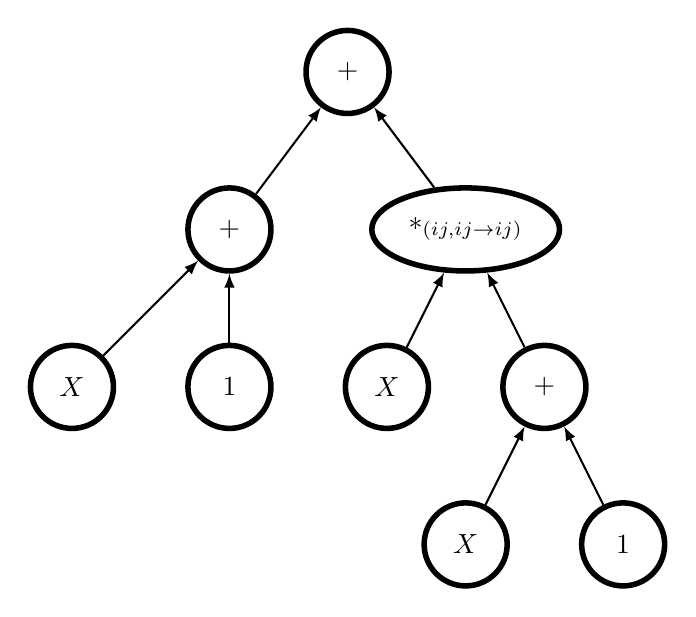
\begin{tikzpicture}[main/.style={draw, circle, minimum size=30pt, line width=2pt}, info/.style={rectangle, rounded corners=5, draw}, n/.style={-latex, line width=0.75pt}, d/.style={-latex, line width=0.75pt, dashed}]
            % nodes
            \node[main] (x1) at (1,0) {$X$};
            \node[main] (11) at (3,0) {$1$};
            \node[main] (+1) at (3,2) {$+$};
            \node[main] (+2) at (4.5,4) {$+$};
            \node[main, shape=ellipse] (*) at (6,2) {$*_{(ij,ij \rightarrow ij)}$};
            \node[main] (x2) at (5,0) {$X$};
            \node[main] (+3) at (7,0) {$+$};
            \node[main] (x3) at (6,-2) {$X$};
            \node[main] (12) at (8,-2) {$1$};
            % edges
            \draw [->, n] (x1) -- (+1);
            \draw [->, n] (11) -- (+1);
            \draw [->, n] (+1) -- (+2);
            \draw [->, n] (*) -- (+2);
            \draw [->, n] (x2) -- (*);
            \draw [->, n] (+3) -- (*);
            \draw [->, n] (x3) -- (+3);
            \draw [->, n] (12) -- (+3);
        \end{tikzpicture}}
    \end{minipage}
    \begin{minipage}{7cm}
        \centering
        \scalebox{0.8}{
        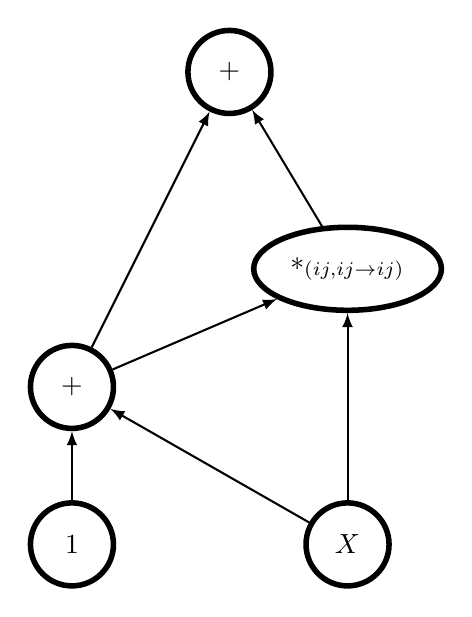
\begin{tikzpicture}[main/.style={draw, circle, minimum size=30pt, line width=2pt}, info/.style={rectangle, rounded corners=5, draw}, n/.style={-latex, line width=0.75pt}, d/.style={-latex, line width=0.75pt, dashed}]
            % nodes
            \node[main] (x1) at (3.5,0) {$X$};
            \node[main] (11) at (0,0) {$1$};
            \node[main] (+1) at (0,2) {$+$};
            \node[main] (+2) at (2,6) {$+$};
            \node[main, shape=ellipse] (*) at (3.5,3.5) {$*_{(ij,ij \rightarrow ij)}$};
            % edges
            \draw [->, n] (x1) -- (+1);
            \draw [->, n] (11) -- (+1);
            \draw [->, n] (+1) -- (+2);
            \draw [->, n] (*) -- (+2);
            \draw [->, n] (x1) -- (*);
            \draw [->, n] (+1) -- (*);
        \end{tikzpicture}}
    \end{minipage}
    \caption{Left: Binary tree generated representing the expression $(X+1) + X *_{(ij,ij \rightarrow ij)} (X+1)$. Right: DAG obtained by eliminating common subtrees in the left tree.}
    \label{fig:tree_to_dag}
\end{figure}
\FloatBarrier
\subsection{Tensor Order Determination}
Another preprocessing step is tensor order determination.
During differentiation, we often create new product nodes.
Because we need to specify product indices when we create a product node, we require knowledge of the tensor orders of both inputs and the output of the new node, which depend on the tensor orders of nodes in the original DAG.
Because we may need the tensor rank of all nodes in the orignal DAG, we determine them by propagating tensor orders from the bottom of the DAG upwards toward the root.

The bottom nodes contain either variables or constants.
The tensor orders of variables need to be given, as they function as the start for the upwards propagation of tensor orders.
Each parent node calculates its tensor order based on its child nodes.
For example, a sum will have its order set equal to the order of its children.
A full overview of these order determination rules can be found in table \ref{tab:order_rules}.

So far we have not addressed how the tensor order of a constant is determined.
Constants may need to be broadcast to fit into the expression.
For example, in the expression $1 + \text{det}(X)$ with an order 2 tensor $X$, $1$ would be a scalar (order 0 tensor) since it needs to be summed with another scalar.
But in the expression $\text{det}(X + 1)$, $1$ would need to be an order 2 tensor filled with ones, because it is summed with another order 2 tensor.
To accomplish this broadcasting, constants have their order set to $-1$ to start with.
Then, when an error is encountered during tensor order determination because an order $-1$ constant does not fit into a part of the expression, the order of the constant is set to the value that makes it fit.

In a sum, this would be the order of the other summand.
In a product, the order would be determined by the given input indices.
In a special function, the order is the input order the function operates on. Since all our special functions operate on matrices, this is always two.
The case of an elementwise function is more difficult, since they operate on arbitrary input tensor orders.
Nonetheless, we may find a fitting order using the expression in which the output of the elementwise function is used, by using the order that is needed there.
This is possible since the input and output order of elementwise functions are always the same.
As an example, the order of the tensor constant $2$ in the expression $X + \text{log}(2)$ may be determined by finding out what order $\text{log}(2)$ needs to be to fit in the sum.
Since summands always have the same order, $\text{log}(2)$, and by extension $2$, need to have the same order as $X$.
Using these rules, we determine the tensor order of any node in an expression DAG.

\begin{table}[ht]
    \centering
    \begin{tabular}{l | l}
        Node Type & Tensor order \\\hline
        \codeword{SUM} & $\text{order}(\text{left}(X))$ \\
        \codeword{PRODUCT} & $\text{output\_indices}(X)$ \\
        \codeword{ELEMENTWISE FUNCTION} & $\text{order}(\text{right}(X))$ \\
        \codeword{adj}, \codeword{inv} & $2$ \\
        \codeword{det} & $0$ \\
    \end{tabular}
    \caption{Rules applied to determine tensor orders of a node $X$, depending on the node's type. Note that the $\text{output\_indices}$ of a product node are given after the $\rightarrow$ in the product string, that the sum may also take its order from the right child, and that each special function (\texttt{det}, \texttt{inv}, \texttt{adj}) needs its own rule.}
    \label{tab:order_rules}
\end{table}

\subsection{Axis Propagation}
In addition to the tensor order, we also require each node to store what its axes are.
The general structure of tensor derivatives is invariant to the specific axis lengths of the tensors variables.
For example, the derivative of $X *_{(ij,ij \rightarrow)} X$ with respect to the order 2 tensor $X$ is always $X + X$ or $2 *_{(,ij \rightarrow ij)} X$, no matter whether $X \in \mathbb{R}^{3 \times 5}$ or $X \in \mathbb{R}^{400 \times 2}$.
This is why we do not require the length of each axis of each variable in a tensor expression to differentiate it.

However, knowing how the shape of each node depends on the shape of the input variables is still useful.
It is necessary for generating program code to numerically compute the derivative we determine and gives us more information about the structure of the derivative.
For these reasons, we do not only propagate tensor order through the input and differentiation DAGs, but also the axes.

First, we give each node a tuple of axes.
Note that we simply use integers to refer to axes in our DAGs.
A node $X$ with tensor order 2 may for example have the axes $(1,2)$, where $1$ and $2$ are simply names for axes, not containing any further information.
In the same way we propagated tensor order, we start from the leaf nodes of the DAG and move toward the top.

In the leaf nodes of the DAG are variables and constants.
Constants start out with no axes while they still have the initial tensor order $-1$.
When a constant gets broadcast, it is assigned fitting axes depending on its surroundings in the expression, in the same way they get fitting tensor orders.

Variables are assigned an $n$-tuple of axes, $n$ being the tensor order of the variable.
Each axis is newly created and not used by any other variable at first.
Then, these axes are propagated upwards through the DAG, using similar rules to the propagation of tensor orders, visible in Table \ref{tab:axes_rules}.

\begin{table}[ht]
    \centering
    \begin{tabular}{l | l}
        Node Type & Axes \\\hline
        \codeword{SUM} & $\text{axes}(\text{left}(X))$ \\
        \codeword{PRODUCT} & See Algorithm \ref{alg:product_axes}\\
        \codeword{ELEMENTWISE FUNCTION} & $\text{axes}(\text{right}(X))$ \\
        \codeword{adj}, \codeword{inv} & $\text{axes}(\text{right}(X))$ \\
        \codeword{det} & $()$ \\
    \end{tabular}
    \caption{Rules applied to determine axes of a node $X$, depending on the type of node it is.}
    \label{tab:axes_rules}
\end{table}

The rule for products is slightly more complex.
It chooses the correct axes for the product node from the axes of its children based on the product index strings.
See Algorithm \ref{alg:product_axes} for further details.

\begin{algorithm}
    \caption{Propagate\_Product\_Axes\_Bottom\_Up (\textit{node})}
    \label{alg:product_axes}
    \begin{algorithmic}
        \For{each \textit{i} in output\_indices(\textit{node})}
            \If{\textit{i} is in left\_indices(\textit{node})}
                \State \textit{p} $\gets$ position of \textit{i} in left\_indices(\textit{node})
                \State append axes(left(\textit{node}))[\textit{p}] to axes(\textit{node})
            \ElsIf{\textit{i} is in right\_indices(\textit{node})}
                \State \textit{p} $\gets$ position of \textit{i} in right\_indices(\textit{node})
                \State append axes(right(\textit{node}))[\textit{p}] to axes(\textit{node})
            \EndIf
        \EndFor
    \end{algorithmic}
\end{algorithm}

After this procedure, each node has a fitting tuple of axes.
However, many of these axes with different names are actually the same.
For example, in the expression $A + B$ for two order 2 tensors $A$ and $B$, this procedure may assign $A$ the axis tuple $(1,2)$ and $B$ the axis tuple $(3,4)$.
$A$ and $B$ are assigned different axes even though the sum requires axis 1 to be equal to axis 3 and axis 2 to be equal to axis 4.

This is why we pass through the DAG a second time, going from the top toward the bottom, unifying axes that are the same.
For each node $x$, we set its childrens' axes depending on its own, with different procedures for different node types.

\begin{table}[ht]
    \centering
    \begin{tabular}{l | l | l}
        Node Type & Left Child Axes & Right Child Axes\\\hline
        \codeword{SUM} & $\text{axes}(X)$ & $\text{axes}(X)$ \\
        \codeword{PRODUCT} & See Algorithm \ref{alg:product_axes_2} & See Algorithm \ref{alg:product_axes_2}\\
        \codeword{ELEMENTWISE FUNCTION} &  - & $\text{axes}(X)$  \\
        \codeword{adj}, \codeword{inv} & - & $\text{axes}(X)$ \\
        \codeword{det} & - &$()$ \\
    \end{tabular}
    \caption{Rules applied when propagating axis downward through a DAG. Note that elementwise and special functions have no left child, as we always set their argument to their right child.}
    \label{tab:axes_rules_2}
\end{table}

An overview of the applied propagation rules is seen in Table \ref{tab:axes_rules_2}.
For a product nodes we employ a more complex procedure, setting each child's axes to the node's axes depending on the product indices.
More details may be seen in Algorithm \ref{alg:product_axes_2}.

\begin{algorithm}[ht!] %TODO: Get this to align at the top
    \caption{Propagate\_Product\_Axes\_Top\_Down (\textit{node})}
    \label{alg:product_axes_2}
    \begin{algorithmic}
        \For{each \textit{i} in output\_indices(\textit{node})}
            \State \textit{p} $\gets$ position of \textit{i} in output\_indices(\textit{node})
            \For{each \textit{j} in left\_indices(\textit{node})}
                \State \textit{q} $\gets$ position of \textit{j} in left\_indices(\textit{node})
                \If{\textit{i} = \textit{j}}
                    \State axes(left(\textit{node}))[\textit{q}] $\gets$ axes(\textit{node})[\textit{p}]
                \EndIf
            \EndFor
            \For{each \textit{j} in right\_indices(\textit{node})}
                \State \textit{q} $\gets$ position of \textit{j} in right\_indices(\textit{node})
                \If{\textit{i} = \textit{j}}
                    \State axes(right(\textit{node}))[\textit{q}] $\gets$ axes(\textit{node})[\textit{p}]
                \EndIf
            \EndFor
        \EndFor
        \For{each \textit{i} in left\_indices(\textit{node})} \algorithmiccomment{Unifies equivalent left and right child axes}
            \State \textit{p} $\gets$ position of first occurence of \textit{i} in left\_indices(\textit{node})
            \If{\textit{i} exists in right\_indices(\textit{node})}
                \State \textit{q} $\gets$ position of first occurence of \textit{i} in right\_indices(\textit{node})
                \State \textit{l} $\gets$ axes(left(\textit{node}))[p]
                \State \textit{r} $\gets$ axes(right(\textit{node}))[q]
                \State rename axis \textit{l} to \textit{r} in all nodes of the DAG
            \EndIf
        \EndFor
    \end{algorithmic}
\end{algorithm}

After this second pass through the DAG, each node now contains a fitting tuple of axes, unified as much as possible, with each axis coming from a variable in the original DAG.

\FloatBarrier
\chapter{Differentiation}
The previous chapter was concerned with creating a suitable internal representation for tensor expressions, which turned out to be a directed acyclic graph (DAG).
In this chapter, we use this DAG representation of the expression for the differentiation.
We start by giving some background information on the general differentiation procedure and describe the differentiation rules in theory.
Following that, we elaborate on the details of our implementation of the procedure and the rules and finish by discussing how expressions grow when we differentiate them.


\section{Background}
The theory for differentiating tensor expressions using our Einstein-like notation was developed by Laue, Mitterreiter and Giesen \cite{tensorpaper}.
They developed differentiation rules for DAG representations of tensor expressions based on the Fr\'{e}chet Derivative.
In their work, they present two modes of differentiation, forward and reverse mode.
This thesis utilizes reverse mode.

In reverse mode, the computation traverses the DAG from top to bottom.
The goal is to calculate for each node $v$ the derivative of the whole expression $y$ with respect to $v$.
This value, $\frac{dy}{dv}$, is also called the pullback of $v$.
When traversing the DAG, the pullback is known for each parent node $u$ of $v$, so we may apply the chain rule:

\begin{equation}
    \frac{dy}{dv} = \sum_{u: (v,u) \in E} \frac{dy}{du} \cdot \frac{du}{dv}
    \label{eq:diff}
\end{equation}

where $(v,u) \in E$ means that there is an edge going from $v$ to $u$ in the DAG, which makes $u$ a parent of $v$. 
Note also that $\cdot$ is a placeholder for an appropriate tensor product, which is specified in the differentiation rules. 
This rule allows us to calculate the pullback of $v$ using the known pullbacks of $v$'s parents $u$.
The only new calculation to be done for each node is the derivation of the parent nodes $u$ with respect to $v$, $\frac{du}{dv}$.

The procedure starts with the root node $y$, representing the entire expression, and computes its pullback, which is the derivative with respect to itself.
This pullback is then used to compute the pullback of $y$'s child nodes, which are used to compute their child nodes, continuing recursively until all paths from the top node $y$ to the argument node have been traversed.
The pullback for the node containing the argument is the result of the differentiation, the derivative of the whole expression $y$ with respect to the argument.

In the very first step of the procedure, the derivative of the top node $y$ with respect to itself is computed.
Since $y$ is a tensor-valued function, its derivative is also a tensor.
Specifically, differentiating $y$ with respect to itself means that each entry of the tensor represented by $y$ is differentiated once with respect to all other entries.
Thus, this differentiation creates a new tensor of the same size as $y$ for each entry in $y$, where for each of these tensors, only one entry is $1$, while the rest are $0$, visible in Figure \ref{fig:delta}.
Concretely, if $y$ is an order $n$ tensor, then its derivative is a tensor $\delta_n$ of order $2n$, where
\begin{equation}
    \delta_n[i_1,..,i_{2n}] = 
    \begin{cases}
        1 \quad \text{if} \; (i_1,..,i_n) = (i_{n+1}...i_{2n}) \\
        0 \quad \text{else}
    \end{cases}
    \label{eq:delta}
\end{equation}
\begin{figure}
    $$
    \begin{pmatrix}
        x_1\\
        x_2\\
        x_3
    \end{pmatrix} \quad \quad \quad \quad \quad \quad
    \begin{pmatrix}
        \frac{\partial x_1}{\partial x_1} & \frac{\partial x_2}{\partial x_1} & \frac{\partial x_3}{\partial x_1} \\
        \frac{\partial x_1}{\partial x_2} & \frac{\partial x_2}{\partial x_2} & \frac{\partial x_3}{\partial x_2} \\
        \frac{\partial x_1}{\partial x_3} & \frac{\partial x_2}{\partial x_3} & \frac{\partial x_3}{\partial x_3}
    \end{pmatrix}
    =
    \begin{pmatrix}
        1 & 0 & 0 \\
        0 & 1 & 0 \\
        0 & 0 & 1
    \end{pmatrix}
    $$
    \caption{Left: An order 1 tensor. Right: The derivative of the left tensor with respect to itself, resulting in an order 2 delta tensor.}
    \label{fig:delta}
\end{figure}
Intuitively, the first $n$ indices point to the entry of $y$ that is being differentiated, while the last $n$ indices point to the entry with respect to which we are differentiating.
Only when we differentiate an entry with respect to itself is the result a $1$, otherwise it is $0$.
Tensors that satisfy Equation \ref{eq:delta} are called delta tensors.
Note that we call a delta tensor of order $2n$ by the name $\delta_n$ and not $\delta_{2n}$, because delta tensors may only have even order.
The first node created in the differentiation procedure is always a delta tensor representing the root node $y$ differentiated with respect to itself.

\section{Differentiation Rules}
Having established the basic differentiation procedure, we will now describe the rules used to compute the derivative $\frac{du}{dv}$ for a node $v$ and its parent $u$.
Proofs for the correctness of these rules can be found in the work of Laue, Mitterreiter and Giesen \cite{tensorpaper}.
Since we are computing $\frac{du}{dv}$, the applied rule depends on the type of node $u$ is.

\FloatBarrier
\subsection{Sum Rule}
If $u$ is a sum node, the differentiation is very simple.
In this case, $u$ adds nothing of its own to the pullback of $v$, so the contribution of $u$ to the pullback of $v$ is only $\frac{dy}{du}$.
Thus, when differentiating a sum node that is their childrens only parent, like the one seen in Figure \ref{fig:sum_rule}, the pullback of the children is simply the pullback of the sum node.

\begin{figure}
    \centering
    \scalebox{0.8}{
        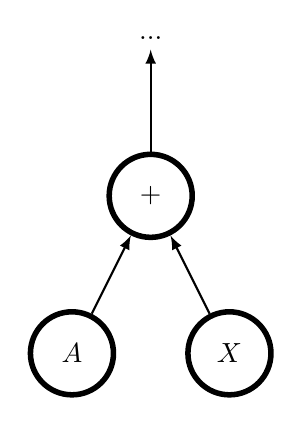
\begin{tikzpicture}[main/.style={draw, circle, minimum size=30pt, line width=2pt}, info/.style={rectangle, rounded corners=5, draw}, n/.style={-latex, line width=0.75pt}, d/.style={-latex, line width=0.75pt, dashed}]
            % nodes
            \node[]  (dots) at (1,4) {...};
            \node[main] (A) at (0,0) {$A$};
            \node[main] (X) at (2,0) {$X$};
            \node[main] (+) at (1,2) {$+$};
            % edges
            \draw [->, n] (A) -- (+);
            \draw [->, n] (X) -- (+);
            \draw [->, n] (+) -- (dots);
        \end{tikzpicture}
    }
    \caption{A sum node in an expression DAG. The pullbacks of its children $A$ and $X$ are the same as its pullback.}
    \label{fig:sum_rule}
\end{figure}

\FloatBarrier
\subsection{Product Rule}
If $u$ is a product node representing the subexpression $v *_{(s_1,s_2 \rightarrow s_3)} w$ with index strings $s_1$, $s_2$ and $s_3$ in a tensor expression where the root node has indices $s_4$, then we may apply the product rule as follows.
The contribution of $u$ to the pullback of $v$ is 
$$
\frac{dy}{du} *_{(s_4s_3,s_2 \rightarrow s_4s_1)} w,
$$
and the contribution to the pullback of $w$ is 
$$
\frac{dy}{du} *_{(s_4s_3,s_1 \rightarrow s_4s_2)} v.
$$
An example of how the product rule is applied to an expression DAG can be seen in Figure \ref{fig:prod_rule}.
There is a caveat to the product rule, because by itself it is not applicable to all tensor products.
This detail will be discussed further in section 4.6.

\begin{figure}
    \centering
    \begin{minipage}{7cm}
        \centering
        \scalebox{0.8}{
            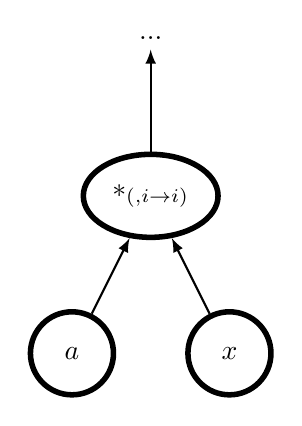
\begin{tikzpicture}[main/.style={draw, circle, minimum size=30pt, line width=2pt}, info/.style={rectangle, rounded corners=5, draw}, n/.style={-latex, line width=0.75pt}, d/.style={-latex, line width=0.75pt, dashed}]
                % nodes
                \node[]  (dots) at (1,4) {...};
                \node[main] (a) at (0,0) {$a$};
                \node[main] (x) at (2,0) {$x$};
                \node[main, ellipse] (*) at (1,2) {$*_{(, i \rightarrow i)}$};
                % edges
                \draw [->, n] (a) -- (*);
                \draw [->, n] (x) -- (*);
                \draw [->, n] (*) -- (dots);
            \end{tikzpicture}
        }
    \end{minipage}
    \begin{minipage}{7cm}
        \centering
        \scalebox{0.8}{
            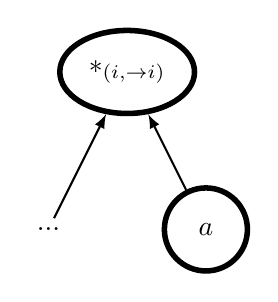
\begin{tikzpicture}[main/.style={draw, circle, minimum size=30pt, line width=2pt}, info/.style={rectangle, rounded corners=5, draw}, n/.style={-latex, line width=0.75pt}, d/.style={-latex, line width=0.75pt, dashed}]
                % nodes
                \node[]           (dots) at (0,0) {...};
                \node[main, ellipse] (*) at (1,2) {$*_{(i, \rightarrow i)}$};
                \node[main]          (a) at (2,0) {$a$};
                % edges
                \draw [->, n] (dots) -- (*);
                \draw [->, n] (a) -- (*);
            \end{tikzpicture}
        }
    \end{minipage}
    \caption{\textbf{Left}: A product node representing a scalar-vector-product in an expression DAG. "..." represents the rest of the DAG. \textbf{Right}: Derivative of the left DAG with respect to $x$ computed using the product rule. "..." represents the pullback of the product node. Note that the product indices in the right DAG depend on the indices $s_4$ of the root node in the left DAG (not visible here), which is assumed to be scalar in this case.}
    \label{fig:prod_rule}
\end{figure}

\FloatBarrier
\subsection{Function Rules}
If $u$ is a function node, we distinguish between two cases.
The node $u$ either represents an elementwise function or a special function.
The elementwise case allows for a slight simplification over the special function case.

If the node $u$ represents an elementwise function $f$ being applied to the child node $v$, then the contribution of $u$ to the pullback of $v$ is 
$$
\frac{dy}{du} *_{(s_2s_1,s_1 \rightarrow s_2s_1)} f'(v),
$$
where $s_1$ is the index string of $v$, $s_2$ is the index string of the output node of the DAG and $f'$ is the derivative of $f$.
An example can be seen in Figure \ref{fig:func_rule}.

If the node $u$ represents a special function $f$ being applied to the child node $v$, then the contribution of $u$ to the pullback $v$ is
$$
\frac{dy}{du} *_{(s_3s_2,s_2s_1 \rightarrow s_3s_1)} f'(v),
$$
where $s_1$ is $v$'s input, representing the domain of $f$, $s_2$ is the index string of $v$, representing the range of $f$, and $s_3$ is the index string of the output node of the DAG with $f'$ still being the derivative of $f$.
The distinction between $s_1$ and $s_2$ is neccessary because domain and range of $f$ may not be the same with these functions.

The derivatives $f'$ of all accepted functions $f$ need to be known.
They are listed in Table \ref{tab:func_diffs}
\begin{table}[ht]
    \centering
    \begin{tabular}{l | l}
        Function & Derivative wrt. x \\\hline
        $-(x)$ & $-(1)$ \\
        $\text{sin}(x)$ & $\text{cos}(x)$ \\
        $\text{cos}(x)$ & $-(\text{sin}(x))$ \\
        $\text{tan}(x)$ & $1 ./ (\text{cos}(x) .^* \text{cos}(x))$ \\
        $\text{arcsin}(x)$ & $1 ./ (1 + -(x .^* x))^{0.5}$ \\
        $\text{arccos}(x)$ & $-(1 ./ (1 + -(x .^* x))^{0.5})$ \\
        $\text{arctan}(x)$ & $1 ./ (1 + (x .^* x))$ \\
        $\text{exp}(x)$ & $\text{exp}(x)$ \\
        $\text{log}(x)$ & $1 ./ x$ \\
        $\text{tanh}(x)$ & $1 + -(\text{tanh}(x) .^* \text{tanh}(x))$ \\
        $\text{abs}(x)$ & $\text{sign}(x)$ \\
        $\text{sign}(x)$ & $0$ \\
        $\text{relu}(x)$ & $\text{relu}(\text{sign}(x))$ \\
        $1 ./ x$ & $- (1 ./ (x .^* x))$ \\
        $\text{inv}(x)$ & $-(\text{inv}(x)) *_{(ij,kl \rightarrow iklj)} \text{inv}(x)$ \\
        $\text{det}(x)$ & $\text{adj}(x) *_{(ij, \rightarrow ji)} 1$ \\
    \end{tabular}
    \caption{Derivatives of all used functions. $.^*$ is a placeholder for elementwise multiplication with the fitting indices. The elementwise inverse $1 ./ x$ is internally handled as an elementwise function, which is why its derivative is listed here.} %TODO: Add a source?
    \label{tab:func_diffs}
\end{table}


\begin{figure}
    \centering
    \begin{minipage}{7cm}
        \centering
        \scalebox{0.8}{
            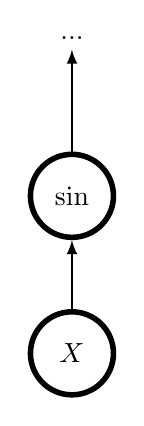
\begin{tikzpicture}[main/.style={draw, circle, minimum size=30pt, line width=2pt}, info/.style={rectangle, rounded corners=5, draw}, n/.style={-latex, line width=0.75pt}, d/.style={-latex, line width=0.75pt, dashed}]
                % nodes
                \node[]    (dots) at (0,4) {...};
                \node[main] (sin) at (0,2) {$\text{sin}$};
                \node[main] (x) at (0,0) {$X$};
                % edges
                \draw [->, n] (x) -- (sin);
                \draw [->, n] (sin) -- (dots);
            \end{tikzpicture}
        }
    \end{minipage}
    \begin{minipage}{7cm}
        \centering
        \scalebox{0.8}{
            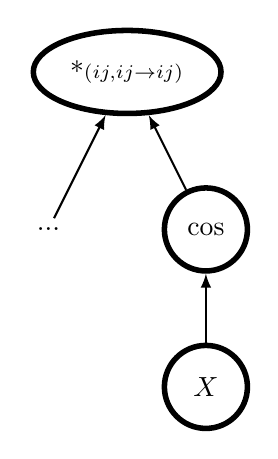
\begin{tikzpicture}[main/.style={draw, circle, minimum size=30pt, line width=2pt}, info/.style={rectangle, rounded corners=5, draw}, n/.style={-latex, line width=0.75pt}, d/.style={-latex, line width=0.75pt, dashed}]
                % nodes
                \node[]           (dots) at (0,0) {...};
                \node[main, ellipse] (*) at (1,2) {$*_{(ij, ij \rightarrow ij)}$};
                \node[main]          (cos) at (2,0) {$\text{cos}$};
                \node[main]          (x) at (2,-2) {$X$};
                % edges
                \draw [->, n] (dots) -- (*);
                \draw [->, n] (cos) -- (*);
                \draw [->, n] (x) -- (cos);
            \end{tikzpicture}
        }
    \end{minipage}
    \caption{\textbf{Left}: Part of a DAG that contains the subexpression $\text{sin(X)}$. $X$ is an order 2 tensor (matrix) and "..." represents the rest of the DAG. \textbf{Right}: Derivative of the left DAG with respect to $X$ computed using the rule for elementwise functions. "..." represents the pullback of the function node. Note that the root output node of the left DAG is assumed to be scalar here, which has an impact on the indices in the product node in the right DAG.}
    \label{fig:func_rule}
\end{figure}

\FloatBarrier
\section{First Example}
In this section, we present a detailed example of the differentiation procedure.
Consider the simple DAG in Figure \ref{fig:diff_example_original}, representing the expression $X *_{(ij,ij \rightarrow ij)} X$, the elementwise product of a matrix $X$ with itself.
We will be differentiating this DAG with respect to $X$.
Each step of the process is visualized in Figure \ref{fig:diff_example_steps}.

Following the differentiation procedure, we start by differentiating the root node with respect to itself.
Since the expression is an order-2 tensor, this creates a delta tensor $\delta_2$ of order 4. (Step 1 in Figure \ref{fig:diff_example_steps})

Continuing from the root node, we compute its contribution to the pullback of the left child first.
In this case, the left child and the right child are the same, but are still handled separately.
Using the product rule, we can see that the contribution of the top node $y$ to the left child is $\frac{dy}{dy} *_{(abij,ij \rightarrow abij)} X$, with $\frac{dy}{dy}$ being $\delta_2$. (Step 2 in Figure \ref{fig:diff_example_steps})

Since $X$ has no children, we continue with the right child of $y$.
Here, we apply the product rule and obtain the same $\delta_2 *_{(abij,ij \rightarrow abij)} X$ as the contribution to the pullback of $X$.
As contributions to the pullbacks of the same node need to be added (see Equation \ref{eq:diff}), we add a sum node as the root of our differentiation DAG. (Step 3 in Figure \ref{fig:diff_example_steps})
Because all ways from the root node to the argument have been processed, we are finished.

\begin{figure}
    \centering
    \scalebox{0.8}{
        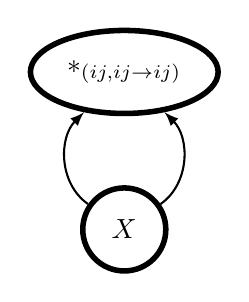
\begin{tikzpicture}[main/.style={draw, circle, minimum size=30pt, line width=2pt}, info/.style={rectangle, rounded corners=5, draw}, n/.style={-latex, line width=0.75pt}, d/.style={-latex, line width=0.75pt, dashed}]
            % nodes
            \node[main] (X) at (0,0) {$X$};
            \node[main, ellipse] (*) at (0,2) {$*_{(ij,ij \rightarrow ij)}$};
            % edges
            \draw [->, n] (X) to[out=145, in=-135] (*);
            \draw [->, n] (X) to[out=35, in=-45] (*);
        \end{tikzpicture}
    }
    \caption{Expression DAG representing the elementwise product of a matrix $X$ with itself.}
    \label{fig:diff_example_original}
\end{figure}

\begin{figure}
    \centering
    \scalebox{0.8}{
        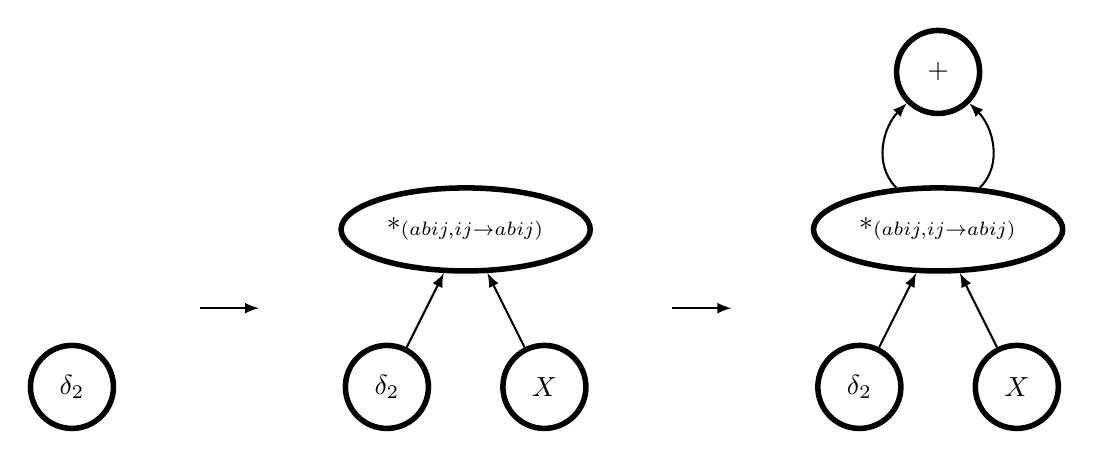
\begin{tikzpicture}[main/.style={draw, circle, minimum size=30pt, line width=2pt}, info/.style={rectangle, rounded corners=5, draw}, n/.style={-latex, line width=0.75pt}, d/.style={-latex, line width=0.75pt, dashed}]
            % nodes
            \node[main] (1delta1) at (0,0) {$\delta_2$};

            \node[] (arr11) at (1.5,1) {};
            \node[] (arr12) at (2.5,1) {};

            \node[main] (1delta1) at (4,0) {$\delta_2$};
            \node[main] (1x1) at (6,0) {$X$};
            \node[main, ellipse] (1*1) at (5,2) {$*_{(abij,ij \rightarrow abij)}$};

            \node[] (arr21) at (7.5,1) {};
            \node[] (arr22) at (8.5,1) {};

            \node[main] (3delta1) at (10,0) {$\delta_2$};
            \node[main] (3x1) at (12,0) {$X$};
            \node[main, ellipse] (3*1) at (11,2) {$*_{(abij,ij \rightarrow abij)}$};
            \node[main] (3+) at (11,4) {$+$};
            % edges
            \draw [->, n] (1delta1) -- (1*1);
            \draw [->, n] (1x1) -- (1*1);

            \draw [->, n] (3delta1) -- (3*1);
            \draw [->, n] (3x1) -- (3*1);
            \draw [->, n] (3*1) to[out=135, in=-135] (3+);
            \draw [->, n] (3*1) to[out=45, in=-45] (3+);

            \draw [->, n] (arr11) -- (arr12);
            \draw [->, n] (arr21) -- (arr22);
        \end{tikzpicture}
    }
    \caption{Progression of the differentiation procedure on the DAG in Figure \ref{fig:diff_example_original}. Left: Pullback of the root node. Middle: One contribution to the pullback of $X$. Right: Pullback of $X$, both contributions summed.}
    \label{fig:diff_example_steps}
\end{figure}

\FloatBarrier
\section{Implementation}
In this chapter we describe how the reverse mode differentiation procedure is implemented using the DAG representation of tensor expressions and the differentiation rules introduced in the previous sections.

An overview of the differentiation procedure can be seen in Algorithm \ref{alg:1} and Algorithm \ref{alg:2}.
The details will be explained in the following paragraphs.

\begin{algorithm}
    \caption{Differentiate (\textit{root}, \textit{argument})}\label{alg:1}
    \begin{algorithmic}
        \State \textit{diffdag} $\gets$ delta(order(\textit{root})) \algorithmiccomment{Creates a node representing $\delta_{\text{order}(root)}$} \\
        \Return ReverseModeDiff(\textit{root}, \textit{argument}, \textit{diffdag}, EmptyDictionary())
    \end{algorithmic}
\end{algorithm}

\begin{algorithm}
    \caption{ReverseModeDiff (\textit{node}, \textit{argument}, \textit{diffdag}, \textit{contributions})}\label{alg:2}
    \begin{algorithmic}
        \For{each \textit{child} of \textit{node}}
            \If{subtree of \textit{child} does not contain \textit{argument}}
                \State Continue with next \textit{child}
            \EndIf
            \State Apply fitting differentiation rule (depending on \textit{node}) to \textit{child}
            \If{\textit{child} is in keys(\textit{contributions})}
                \State Add new contribution to \textit{contributions}[\textit{child}] using a sum node
                \State Move all parents of the \textit{contributions}[\textit{child}] to the sum node
                \State Update \textit{contributions}[\textit{child}] as the sum node
            \Else
                \State \textit{contributions}[\textit{child}] $\gets$ \textit{diffdag}
                \State \textit{diffdag} $\gets$ ReverseModeDiff(\textit{child}, \textit{argument}, \textit{diffdag}, \textit{contributions})
            \EndIf
        \EndFor \\
        \Return diffdag
    \end{algorithmic}
\end{algorithm}

As can be seen in Algorithm \ref{alg:1}, the first node is added specially, before the real differentiation algorithm starts.
This node, a delta tensor, is the derivative of the top node $y$ with respect to itself and has double the order of the original top node.

The original DAG is traversed from the top node down to the argument node, building up the differentiation DAG alongside it.
With each node $u$ of the original DAG that is processed, its contributions to the pullbacks of its child nodes are added to the differentiation DAG.
These pullbacks are computed using the differentiation rules discussed in the previous chapter.

As we are operating on a DAG and not a tree, a single node may be reached multiple times during differentiation.
When differentiating a node $u$, one of its children $v$ may have already been reached through a different parent.
In this case, a part of the pullback of $v$ has already been computed and is present in the differentiation DAG.
The new pullback contribution we computed from $u$ needs to be added to the old part, as can be seen from Equation \ref{eq:diff}.
To be able to do this, we keep a dictionary mapping from nodes in the original DAG which we have already reached to their pullback in the differentiation DAG.
This lets us add the old and new pullback contributions with a sum node.
Afterwards, we update the entry in the dictionary to the sum node that was just added so that further contributions are added there.
We also need to move all nodes in the differentiation DAG that rely on the pullback of $v$, specifically the parents.
Thus, we set all parents of the old pullback to have the updated pullback as their child.
This way, we build up the correct pullback over time, adding contributions as we find new ways to reach each node.

\FloatBarrier
\section{Second Example}
To better illustrate the process of building a pullback piece by piece, we showcase an example.
Consider the DAG in Figure \ref{fig:alg_example_1} representing the expression $\text{sin}(v) + \text{cos}((\text{sin}(v)))$ for an order 1 tensor $v$.
We differentiate this expression with respect to $v$.

Starting out, we compute the pullback of the root node.
Since the output of the root node is an order 1 tensor, its pullback, the derivative with respect to itself, is an order 2 delta tensor $\delta_1$. (Step 1 in Figure \ref{fig:alg_example_2})

Next, we compute the contribution of the root node to its children's pullbacks.
However, since the root node is a sum node, it adds nothing of its own, which makes its childrens pullbacks the same as its.

Continuing with the node's children, we start (arbitrarily) with the left child.
The left child is an elementwise function node representing $\text{sin}(v)$.
Using the differentiation rule for elementwise functions along with the derivative of the $\text{sin}$ function, we see that its contribution to its child's pullback is $\delta_1 *_{(ba,a \rightarrow ba)} \text{cos}(v)$.
This is the first contribution to the pullback of $v$. (Step 2 in Figure \ref{fig:alg_example_2})
Since the only child of the $\text{sin}$ node is the argument node $v$, we need not continue further and instead jump back up to explore the second child of the root node.

The second child is an elementwise function node representing $\text{cos}((\text{sin}(v)))$.
Using the differentiation rule for elementwise functions along with the derivative of the $\text{cos}$ function, we obtain $\delta_1 *_{(ba,a \rightarrow ba)} -(\text{sin}(v))$ as the contribution of the node to its child's pullback.

The $\text{cos}$ node's child is the $\text{sin}$ node we have been to before.
This means we need to add the new contribution to this node's pullback to the old one.
The old contribution to the pullback of $\text{sin}(v)$ was $\delta_1$, to which we now add $\delta_1 *_{(ba,a \rightarrow ba)} -(\text{sin}(v))$ using a sum node.
Since the pullback of $v$ depends on the pullback of $\text{sin}(v)$, we need to make sure to update it.
We manage this by moving all parents of the old pullback to be parents of the new pullback instead.
The left child of the product $\delta_1 *_{(ba,a \rightarrow ba)} \text{cos}(v)$ gets updated to be the sum node in the new, complete pullback. (Step 3 in Figure \ref{fig:alg_example_2})

Since there are no more unvisited children, we are done.
The finished differentiation DAG represents the expression $(\delta_1 + (\delta_1 *_{(ba,a \rightarrow ba)} -(\text{sin}(v)))) *_{(ba,a \rightarrow ba)} cos(v)$.
The complete, simplified DAG is visible in Figure \ref{fig:alg_example_3}.

\begin{figure}
    \centering
    \scalebox{0.8}{
        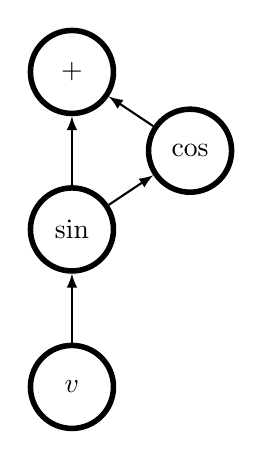
\begin{tikzpicture}[main/.style={draw, circle, minimum size=30pt, line width=2pt}, info/.style={rectangle, rounded corners=5, draw}, n/.style={-latex, line width=0.75pt}, d/.style={-latex, line width=0.75pt, dashed}]
            % nodes
            \node[main] (v) at (0,0) {$v$};
            \node[main] (sin) at (0,2) {$\text{sin}$};
            \node[main] (cos) at (1.5,3) {$\text{cos}$};
            \node[main] (+) at (0,4) {+};
            % edges
            \draw [->, n] (v) -- (sin);
            \draw [->, n] (sin) -- (+);
            \draw [->, n] (sin) -- (cos);
            \draw [->, n] (cos) -- (+);
        \end{tikzpicture}
    }
    \caption{DAG representing the expression $\text{sin}(v) + \text{cos}((\text{sin}(v)))$.}
    \label{fig:alg_example_1}
\end{figure}


\begin{figure}
    \centering
    \scalebox{0.8}{
        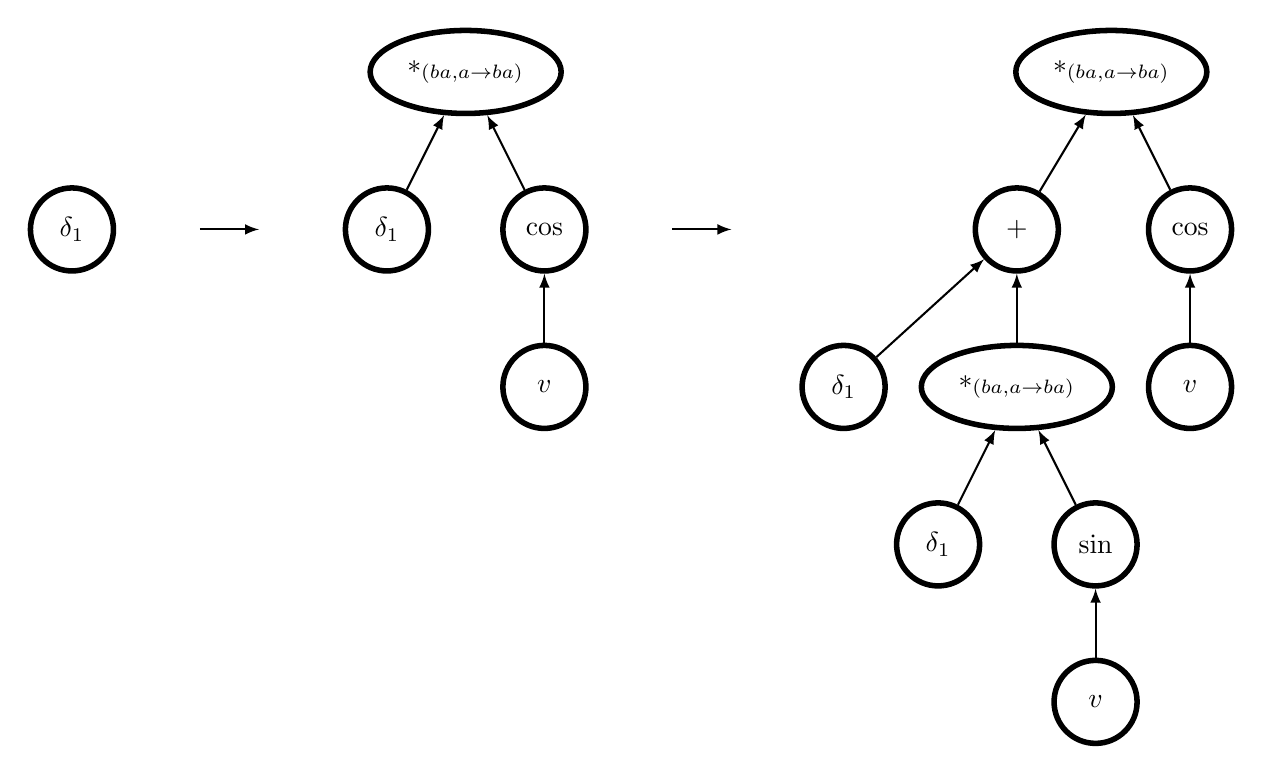
\begin{tikzpicture}[main/.style={draw, circle, minimum size=30pt, line width=2pt}, info/.style={rectangle, rounded corners=5, draw}, n/.style={-latex, line width=0.75pt}, d/.style={-latex, line width=0.75pt, dashed}]
            % nodes
            \node[main] (1delta) at (0,2) {$\delta_1$};

            \node[] (arr11) at (1.5,2) {};
            \node[] (arr12) at (2.5,2) {};

            \node[main] (2v) at (6,0) {$v$};
            \node[main] (2cos) at (6,2) {$\text{cos}$};
            \node[main] (2delta) at (4,2) {$\delta_1$};
            \node[main, ellipse] (2*1) at (5,4) {$*_{(ba,a \rightarrow ba)}$};

            \node[] (arr21) at (7.5,2) {};
            \node[] (arr22) at (8.5,2) {};
            
            \node[main] (3v) at (14.2,0) {$v$};
            \node[main] (3cos) at (14.2,2) {$\text{cos}$};
            \node[main, ellipse] (3*1) at (13.2,4) {$*_{(ba,a \rightarrow ba)}$};
            \node[main] (3+) at (12,2) {$+$};
            \node[main, ellipse] (3*2) at (12,0) {$*_{(ba,a \rightarrow ba)}$};
            \node[main] (3sin) at (13,-2) {$\text{sin}$};
            \node[main] (3v2) at (13,-4) {$v$};
            \node[main] (3delta1) at (11,-2) {$\delta_1$};
            \node[main] (3delta2) at (9.8,0) {$\delta_1$};
            % edges
            \draw [->, n] (2v) -- (2cos);
            \draw [->, n] (2cos) -- (2*1);
            \draw [->, n] (2delta) -- (2*1);

            \draw [->, n] (3v) -- (3cos);
            \draw [->, n] (3cos) -- (3*1);
            \draw [->, n] (3+) -- (3*1);
            \draw [->, n] (3*2) -- (3+);
            \draw [->, n] (3sin) -- (3*2);
            \draw [->, n] (3v2) -- (3sin);
            \draw [->, n] (3delta1) -- (3*2);
            \draw [->, n] (3delta2) -- (3+);

            \draw [->, n] (arr11) -- (arr12);
            \draw [->, n] (arr21) -- (arr22);
        \end{tikzpicture}
    }
    \caption{Progression of the differentiation procedure on the DAG in Figure \ref{fig:alg_example_1}. Left: Pullback of the $+$, $\text{sin}$ and $\text{cos}$ nodes. Middle: First contribution to the pullback of $v$. Right: Full pullback of $v$.}
    \label{fig:alg_example_2}
\end{figure}

\begin{figure}
    \centering
    \scalebox{0.8}{
        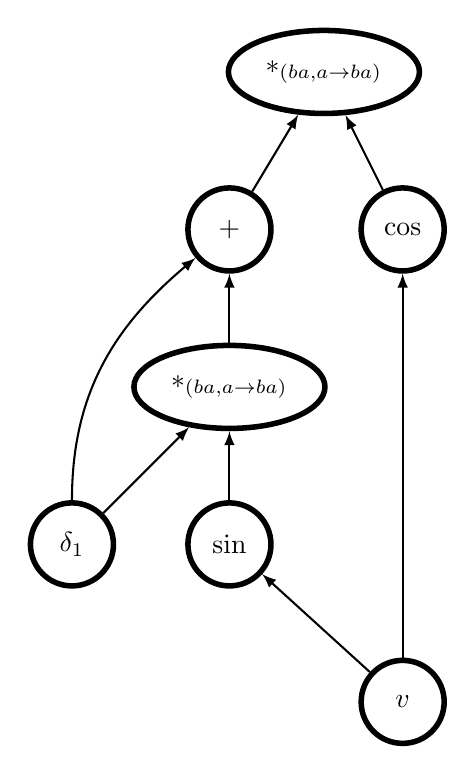
\begin{tikzpicture}[main/.style={draw, circle, minimum size=30pt, line width=2pt}, info/.style={rectangle, rounded corners=5, draw}, n/.style={-latex, line width=0.75pt}, d/.style={-latex, line width=0.75pt, dashed}]
            % nodes
            \node[main] (v) at (2.2,-4) {$v$};
            \node[main] (cos) at (2.2,2) {$\text{cos}$};
            \node[main, ellipse] (*1) at (1.2,4) {$*_{(ba,a \rightarrow ba)}$};
            \node[main] (+) at (0,2) {$+$};
            \node[main, ellipse] (*2) at (0,0) {$*_{(ba,a \rightarrow ba)}$};
            \node[main] (sin) at (0,-2) {$\text{sin}$};
            \node[main] (delta) at (-2,-2) {$\delta_1$};
            % edges
            \draw [->, n] (v) -- (cos);
            \draw [->, n] (cos) -- (*1);
            \draw [->, n] (+) -- (*1);
            \draw [->, n] (*2) -- (+);
            \draw [->, n] (sin) -- (*2);
            \draw [->, n] (v) -- (sin);
            \draw [->, n] (delta) -- (*2);
            \draw [->, n] (delta) to[out=90, in=220] (+);
        \end{tikzpicture}
    }
    \caption{Full simplified differentiation DAG of the original DAG in Figure \ref{fig:alg_example_1}.}
    \label{fig:alg_example_3}
\end{figure}

\FloatBarrier
\section{Invalid Nodes Created by the Product Rule}
In this section we present a problem with the differentiation of tensor products that was discovered during development, along with a solution.

\subsection{Problem}
We discovered that the differentiation rule for products sometimes creates invalid product nodes.
Specifically in the case where an index appears only in the index string of exactly one input of a product node, but not in the output index string.
An example of this would be the left DAG in Figure \ref{fig:missing_indices_example}, containing a node representing the product $A *_{(ij,j \rightarrow )} v$, where the index $i$ only appears in the left index string.
When differentiating this DAG with respect to $A$, we compute the contribution of the product node to the pullback of $A$ and receive $\delta_0 *_{(,j \rightarrow ij)} v$ using the product rule.
The resulting product node is not valid, because the index $i$ appears in the result index string, but not in either input index string.

The root of this problem can be found in the proof of the reverse mode differentiation product rule in the work \cite{tensorpaper} by Laue, Mitterreiter and Giesen (Theorem 8).
In this proof, Laue, Mitterreiter and Giesen find the derivative of a product node $A *_{(s_1, s_2 \rightarrow s_3)} B$ with respect to $B$, although all statements we make are analogously applicable to the differentiation with respect to $A$.
They utilize the Fr\'{e}chet Derivative, which is defined as follows.

For a function $f$ that maps from an order $k$ tensor to an order $l$ tensor, we call a tensor $D$ of order $k+l$ the derivative of $f$ at $x$ if and only if
$$
\text{lim}_{h \rightarrow 0} \frac{||f(x+h) - f(x) - D \circ h||}{||h||} = 0
$$
Here, $\circ$ describes an inner product.
In our notation, an inner product has the form $D *_{(s_1 s_2, s_2 \rightarrow s_1)} h$ for two index strings $s_1$ and $s_2$.

Mittereiter, Laue and Giesen start from this definition applied to the product node $A *_{(s_1, s_2 \rightarrow s_3)} B$ and transform it to describe the pullback of $B$.
Important to us is the fourth equality of the proof, where the associative property for tensor products is used to transform $\bar{C} *_{(s_4s_3,s_3 \rightarrow s_4)} (A *_{(s_1,s_2 \rightarrow s_3)} h)$ into $(\bar{C} *_{(s_4s_3,s_1 \rightarrow s_4s_2)} A) *_{(s_4s_2,s_2 \rightarrow s_4)} h$.
Their goal is to create an expression that ends with a form of $D \circ h$, because that makes $D$ the Fr\'{e}chet Derivative they are looking for.

Consider however the definition of the associative property for tensor products given by Laue, Mitterreiter and Giesen.
$$
(A *_{(s_1, s_2 s_4 \rightarrow s_3 s_4)} B) *_{(s_3 s_4, s_4 \rightarrow s_3)} C = A *_{(s_1, s_2 \rightarrow s_3)} (B *_{(s_2 s_4, s_4 \rightarrow s_2)})
$$
where $s_3 \subseteq s_1 \cup s_2$ and $s_4 \cap (s_1 \cup s_2) = \emptyset$. 
Applying the associative property to our expression would require that $s_1 = s_3 s_2$, which is not the case for all product nodes.
Thus, we cannot always apply the associative property here.

\subsection{Solution}
To solve this problem, we forego the stated version of the associative property and find another way to transform $\bar{C} *_{(s_4s_3,s_3 \rightarrow s_4)} (A *_{(s_1,s_2 \rightarrow s_3)} h)$ into an inner product.

We start by explicitly writing the Einstein-like tensor products as sums.
The indices we sum over are the indices of the inputs with the result indices removed.
$$
\sum_{s_3} \bar{C}[s_4 s_3] \; (\sum_{s_1 s_2 \setminus s_3} A[s_1] \; h[s_2]) 
$$
Note that we obtain the indices of the outer sum from $s_3 s_4 \setminus s_4 = s_3$.
As both sums go over separate, non-overlapping index sets, we may collapse them into a single sum.
$$
\sum_{s_1 s_2 s_3} \bar{C}[s_4 s_3] \; A[s_1] \; h[s_2]
$$
As the first step towards writing our expression as an inner product, we split off part of the large sum to create two smaller sums over different indices.
$$
\sum_{s_2} (\sum_{s_1 s_3 \setminus s_2} \bar{C}[s_4 s_3] \; A[s_1]) \; h[s_2]
$$
Next, we write the inner sum in our Einstein-like tensor product notation.
This requires us to determine the output indices of the tensor product by adding the input indices, $s_4 s_3$ and $s_1$, and removing the indices that are summed over, $s_1 s_3 \setminus s_2$.
This leads to $s_1 s_3 s_4 \setminus (s_1 s_3 \setminus s_2)$, which we may simplify in the following way:
\begin{align*}
&s_1 s_3 s_4 \setminus (s_1 s_3 \setminus s_2) \\
&= s_1 s_3 s_4 \setminus (s_1 s_3 \cap \overline{s_2}) \\
&= s_1 s_3 s_4 \cap \overline{(s_1 s_3 \cap \overline{s_2})} \\
&= s_1 s_3 s_4 \cap (\overline{s_1 s_3} \cup s_2) \\
&= (s_1 s_3 s_4 \cap \overline{s_1 s_3}) \cup (s_1 s_3 s_4 \cap s_2) \\
&= (s_1 s_3 s_4 \setminus s_1 s_3) \cup (s_1 s_3 s_4 \cap s_2) \\
&= (s_4 \setminus s_1 s_3) \cup (s_1 s_3 s_4 \cap s_2) \\
&= s_4 \cup (s_1 s_3 s_4 \cap s_2) \\
&= s_4 \cup (s_1 s_3 \cap s_2) \\
\end{align*}
where $\bar{x}$ is the set complement of $x$.
The last two simplification steps are possible because the output indices of the root node, $s_4$, are always be chosen to be disjoint to $s_1$, $s_2$ and $s_3$.

With these output indices, we may rewrite our expression.
$$
\sum_{s_2} (C *_{(s_4 s_3, s_1 \rightarrow s_4 \cup (s_1 s_3 \cap s_2))} A) \; h[s_2]
$$
We know that the output indices of this expression need to be $s_4$ from the version we started with.
Using this, we can rewrite the outer sum in our tensor product notation as well.
$$
(C *_{(s_4 s_3, s_1 \rightarrow s_4 \cup (s_1 s_3 \cap s_2))} A) *_{((s_4 \cup (s_1 s_3 \cap s_2)), s_2 \rightarrow s_4)} h
$$
At this point, if we had $s_4 s_2$ instead of $s_4 \cup (s_1 s_3 \cap s_2)$ in the left and right products, the right product would have the form $*_{(s_4 s_2, s_2 \rightarrow s_4)}$ and would be an inner product.
We can see that $s_4 s_2 \neq s_4 \cup (s_1 s_3 \cap s_2)$ when there are indices in $s_2$ that are not present in either $s_1$ or $s_3$.
If we could remove this case, we would be successful in creating an inner product and thus in computing the derivative.

To implement this idea and prevent invalid product nodes from appearing, we modify the original DAG before it is differentiated.
For any product node of the form $A *_{(s_1, s_{21} s_{22} \rightarrow s_3)} B$ where $s_{21} \cap (s_1 s_3) = s_{21}$ and $s_{22} \cap (s_1 s_3) = \emptyset$, we call $s_{22}$ the missing indices of this node and transform the node by making the sum over the missing indices explicit.

We append the missing indices to the output index string of the product node, leading to $A *_{(s_1, s_{21} s_{22} \rightarrow s_3 s_{22})} B$.
This prevents an invalid product node from being created, because the indices in $s_{22}$ are now also present in the output indices.
However, this also changes the node, since it now has more output axes than before.
To remedy this, we add another product node where we explicitly sum over these axes while multiplying with a tensor full of ones, leasing to $(A *_{(s_1, s_{21} s_{22} \rightarrow s_3 s_{22})} B) *_{(s_3 s_{22}, s_{22} \rightarrow s_3)} 1$.
Since $s_3$ appears in both the left input and the output, and $s_{22}$ appears in both inputs, this new product never has any missing indices.
This transformation achieves the same result as the original DAG, but by making the sum over the axes explicit in another product node, we prevent the problematic case.

In the example in Figure \ref{fig:missing_indices_example}, we would transform the original expression from $A *_{(ij,j \rightarrow )} v$ to $(A *_{(ij,j \rightarrow i)} v) *_{(i,i \rightarrow)} 1$.
Both the modified DAG and the derivative are visible in Figure \ref{fig:missing_indices_example}.

\begin{figure}
    \begin{minipage}{4cm}
        \centering
        \scalebox{0.8}{
            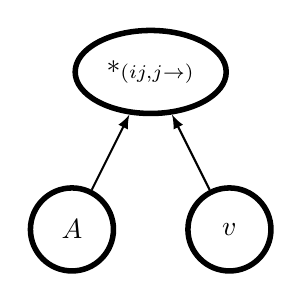
\begin{tikzpicture}[main/.style={draw, circle, minimum size=30pt, line width=2pt}, info/.style={rectangle, rounded corners=5, draw}, n/.style={-latex, line width=0.75pt}, d/.style={-latex, line width=0.75pt, dashed}]
                % nodes
                \node[main] (A) at (0,0) {$A$};
                \node[main] (v) at (2,0) {$v$};
                \node[main, ellipse] (*) at (1,2) {$*_{(ij,j \rightarrow )}$};
                % edges
                \draw [->, n] (A) -- (*);
                \draw [->, n] (v) -- (*);
            \end{tikzpicture}
        }
    \end{minipage}
    \begin{minipage}{5cm}
        \centering
        \scalebox{0.8}{
            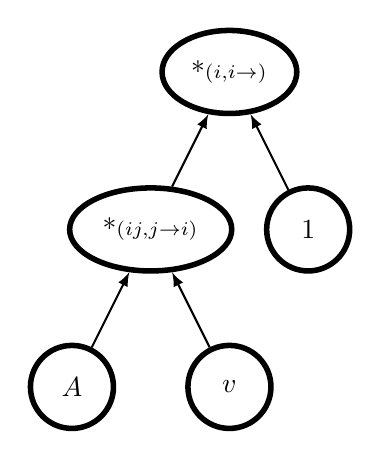
\begin{tikzpicture}[main/.style={draw, circle, minimum size=30pt, line width=2pt}, info/.style={rectangle, rounded corners=5, draw}, n/.style={-latex, line width=0.75pt}, d/.style={-latex, line width=0.75pt, dashed}]
                % nodes
                \node[main] (A) at (0,0) {$A$};
                \node[main] (v) at (2,0) {$v$};
                \node[main, ellipse] (*) at (1,2) {$*_{(ij,j \rightarrow i)}$};
                \node[main] (1) at (3,2) {$1$};
                \node[main, ellipse] (*2) at (2,4) {$*_{(i,i \rightarrow )}$};
                % edges
                \draw [->, n] (A) -- (*);
                \draw [->, n] (v) -- (*);
                \draw [->, n] (*) -- (*2);
                \draw [->, n] (1) -- (*2);
            \end{tikzpicture}
        }
    \end{minipage}
    \begin{minipage}{5cm}
        \centering
        \scalebox{0.8}{
            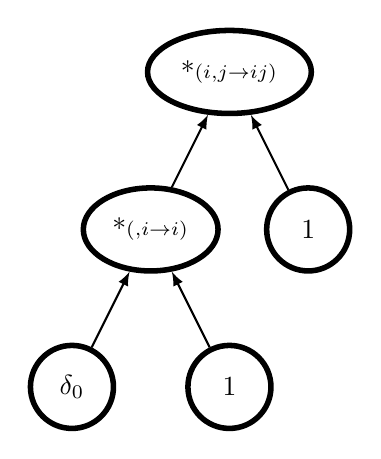
\begin{tikzpicture}[main/.style={draw, circle, minimum size=30pt, line width=2pt}, info/.style={rectangle, rounded corners=5, draw}, n/.style={-latex, line width=0.75pt}, d/.style={-latex, line width=0.75pt, dashed}]
                % nodes
                \node[main] (delta) at (0,0) {$\delta_0$};
                \node[main] (1) at (2,0) {$1$};
                \node[main, ellipse] (*) at (1,2) {$*_{(,i \rightarrow i)}$};
                \node[main] (v) at (3,2) {$1$};
                \node[main, ellipse] (*2) at (2,4) {$*_{(i,j \rightarrow ij)}$};
                % edges
                \draw [->, n] (delta) -- (*);
                \draw [->, n] (1) -- (*);
                \draw [->, n] (*) -- (*2);
                \draw [->, n] (v) -- (*2);
            \end{tikzpicture}
        }
    \end{minipage}
    \caption{Left: DAG with a disappearing index $i$. Middle: Modified DAG where the sum over index $i$ is made explicit. Right: Derivative of the middle DAG with respect to $A$.}
    \label{fig:missing_indices_example}
\end{figure}

\section{Expression Growth}
For performance purposes, it is of interest how the sizes of expressions change when we differentiate them.
The size of an expression DAG may be measured in the number of nodes $|V|$ or the number of edges $|E|$ in the DAG.
We include discussions on both size measures.
In the differentiation process, there are two points where nodes are added to the differentiation DAG: when applying the differentiation rules and when summing contributions to the same pullback.

We apply one differentiation rule per node, with each differentiation rule adding a constant number of nodes and edges to the differentiation DAG.
Thus, the number of nodes and the number of edges both scale linearly ($O(|V|)$) during this step.

When we sum contributions to the pullback of a node $X$, we add one sum node and two edges for each contribution after the first one.
Because each contribution stems from one incoming edge (from a parent node) of $X$, we add one sum node and a constant 2 edges for each incoming edge of $X$ in total.
At most, we add one node and two edges for every edge in the DAG, leading to a growth of $O(|E|)$ both in the number of nodes and edges.

This leads to a total growth in the number of nodes and edges of $O(|V| + |E|)$ from the original expression DAG to the differentiation DAG.
However, since each incoming edge of a node in the DAG represents one occurence of that node in the original unsimplified binary tree, we may also say that the total growth in both the number of nodes and the number of edges is $O(|V|)$ from the original unsimplified binary expression tree to the differentiation DAG.

\chapter{Summary}
In this thesis, we covered the design and implementation of a calculus for automtatic symbolic differentiation of tensor expressions.
We created a language for general tensor expressions using an Einstein-like notation for tensor products and discussed how expressions formulated in this language may be parsed into a suitable representation, a directed acyclic graph (DAG).
We also demonstrated multiple preprocessing steps, substituting some subexpressions for more easily differentiable ones, eliminating multiple occurences of the same subexpression and storing both tensor order and an axis tuple for each node in the DAG.
We gave a review of the theory behind the differentiation of tensor expressions using our notation and demonstrated our implementation, which is able to differentiate the preprocessed expression DAGs.
The correctness of our implementation was verified by numerical checks, where the computed derivatives of a number of example inputs were compared with numerical approximation for random inputs. %TODO: IS THIS OUT-OF-PLACE?
Possible further developments could address the flexibility and readablity of the input language, for example by adding a generalized transpose operation that allows axis permutations, which have to be embedded in tensor products in the current language.
The tensor products could also be generalized even further, possibly by adding a unary version that allows one to sum over a single tensor's axes.
Furthermore, our algorithms could be analyzed and optimized in regards to efficiency and performance for different inputs.
Lastly, one possible use of this thesis' results are convexity checks for arbitrary functions.
How our representation of tensor function derivatives can be used to detect convexity and concavity is worth investigating.
\addcontentsline{toc}{chapter}{Bibliography}
\printbibliography

\addcontentsline{toc}{chapter}{Statement of Autonomy}
\chapter*{Declaration of Authorship}
I hereby declare that I have created this thesis autonomously, using only the stated assistance and sources.
The thesis has not been used for other courses or within other exam processes as exam work, nor has it been published in any language.

\setlength{\parindent}{0pt}
\vspace{10pt}
The author does not object to this thesis being made available for public use. \vspace{50pt}

Jena, 25.08.2022


\end{document}